
\input{../Common/commands}

\begin{document}

\graphicspath{ {../Common/images/} }
\input{../Common/map}
\graphicspath{ {images/} }


% ----------------------------------------------------------------
% PAGE TITLE
% ----------------------------------------------------------------
\title{\headerpres{Data Analysis: \\ Special Topics }}
\author{\vspace{3cm} Institute of Technology Tallaght}
\date{Department of Computing}
\maketitle
\newpage

% ----------------------------------------------------------------
% PAGE 
% ----------------------------------------------------------------
\headerch{Introduction}
The topics covered in this last session are each somewhat different from data analysis as we have studied it so far in this module:
\begin{itemize}
\item Text mining - unstructured data, with data preparation an important part of the process
\item Social network analysis - data in the form of network topology information, including nodes and connections
\item Web mining - a combination of three aspects
  \begin{itemize}
  \item network topology (www structure)
  \item text and media (www content)
  \item usage and user behaviour (www log files)
  \end{itemize}
\end{itemize}

\newpage

\headerch{Text mining}
\begin{itemize}
\item Many and varied sources of data:
  \begin{itemize}
  \item by type: business reports, business communication, online news, personal messaging, standards documents, specialist document archives, scientific literature etc.
  \item by domain: law, science, medicine, business, finance etc.
    \item by format: PDF files, MS Word files, XML files, text messages, tweets etc.
  \end{itemize}
\item Applications:
  \begin{itemize}
  \item \textbf{marketing:}
    \begin{itemize}
      \item 'social personas' clustering technique from customer communication, social media sources, blogs etc.
      \item 'listening platform' for real-time gathering of customer sentiment
      \item analysis of call centre conversations to understand performance and potential problems
    \end{itemize}
  \item \textbf{business operations:}
    \begin{itemize}
    \item analysis of sentiment among employees
    \item general understanding of consumer behaviour and its applications
    \end{itemize}
  \item \textbf{legal:}
    \begin{itemize}
    \item e-discovery platforms that help to minimize risk when sharing documents
    \item analysis of case histories and risk assessment
    \item archive searches for help with case handling based on precedences etc.
    \end{itemize}
  \item \textbf{government and politics:}
    \begin{itemize}
    \item assessment of general population or constituent sentiment 
    \item geopolitical security
    \end{itemize}      
  \end{itemize}
\item Text is unstructured data but we have to start somewhere when analysing it
  \begin{itemize}
  \item Bag of words - in the first instance, a body of text is viewed as a grouping of words, which may be repeated
  \item Every word is a possible attribute, but what value can we give it for a document?
    \begin{itemize}
    \item 1 vs 0 - depending on whether the word is present in the document or not
    \item count - representing the number of times the word appears in the document - results in a term-document-table:\\
      \begin{tabular}{ccccc}
        & why & where & how & the \\
        \hline
        doc1 & 3 & 2 &0 & 7 \\ 
        doc2 & 1 & 0 &2 & 10 \\ 
        doc3 & 0 & 1 &1 & 10 \\ 
      \end{tabular}
    \item normalization (lowercase, only roots, stopwords removed, division by number of words if multiple documents)\\
      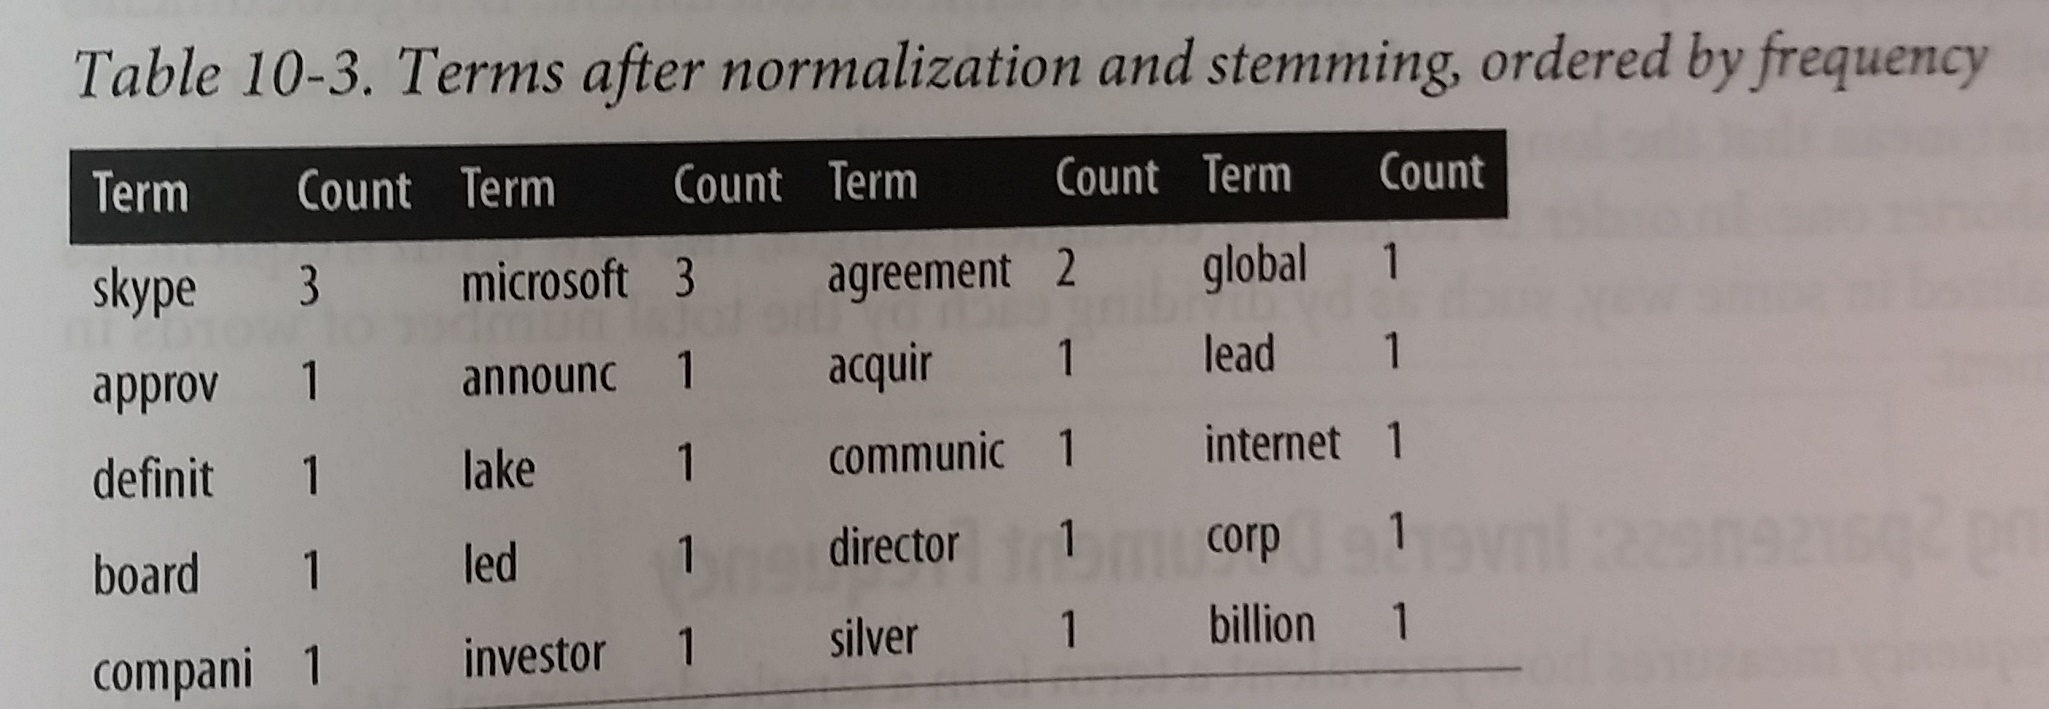
\includegraphics[width=0.5\textwidth]{norm_tdt.jpg}
    \end{itemize}
  \end{itemize}
\item What for?
  \begin{itemize}
  \item incidence of words (e.g. word-cloud)
  \item predicting chances of a document being liked based on comparison with previous documents (predictive modelling)
  \item clustering for determining document type, sentiment etc.
    \item association rule analysis e.g. word 'happy' occurs with what other words?
  \end{itemize}
\end{itemize}

\newpage


\headerch{Social network analysis}
\begin{itemize}
\item Applications:
  \begin{itemize}
  \item study of communities 
  \item marketing
  \item public health (disease spread)
  \item human behaviour and self awareness
  \end{itemize}
\item Differs from data analysis in general because it is based around analysing network topologies and their properties:
  \begin{itemize}
  \item ring / hub and spokes \\
    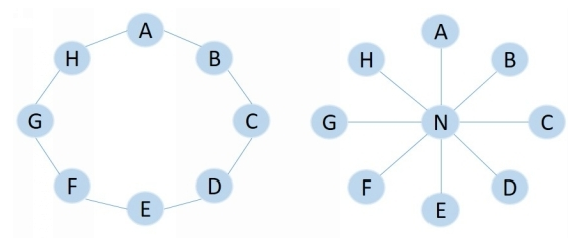
\includegraphics[width=0.5\textwidth]{hub_spoke.png}
  \item sparse / dense
  \item subnetworks\\
    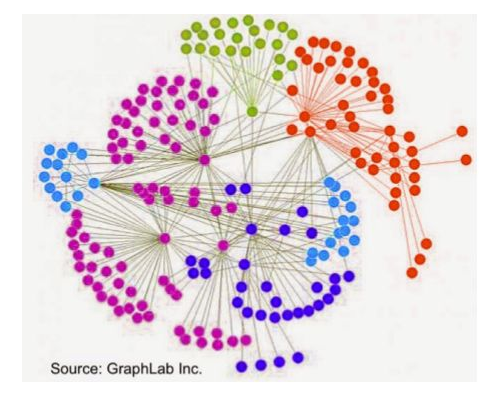
\includegraphics[width=0.5\textwidth]{subnet.png}
  \item node importance (+)
  \end{itemize}
  \item Google page rank (85\% importance and 15\% Teleporting)
\end{itemize}
\newpage

\headerch{Web mining}
\begin{itemize}
\item Content mining (HTML etc)
\item Structure mining (hyperlinks resulting in network topology)
\item Usage (site visits, clicks)
\end{itemize}
\newpage



\end{document}
